\section{Modular functions}

We devote the last section of this thesis to the visualization of modular functions. The theory of modular functions is a branch of complex analysis whose importance and beauty lies most notably in its connections to number theory. We will however not dive deeply into this theory. Instead we will content ourselves with depicting graphs of certain selected modular functions, enjoying their visual aesthetics and reading off some of its properties, like zeros and poles as well as their order. Unfortunately such illustrations of modular functions are rarely found in literature. Therefore this section should be considered as complementary material to more comprehensive treatments on the theory of modular functions given for example in \Klein{}, \Lehner{} or \Schoeneberg{}.

\index{Meromorphic function}
Modular functions are meromorphic maps (\ie maps which are holomorphic\footnote{Holomorphic functions are also frequently called ``analytic''.} except for isolated poles, or in other words, maps which can be represented as quotient of two holomorphic functions) which are defined on the upper half-plane and which are invariant under the transformations of the modular group.

\begin{definition}[Modular function]
Let the upper halfplane $\mathcal{H}$ and the extended upper halfplane $\EU$ be defined as in (\ref{eqn_Upperhalfplane}) and (\ref{eqn_ExtUpperhalfplane}) respectively.
A map $F : \EU \to \EC$ is called a \emph{modular function}, if it satisfies the following conditions:
\begin{enumerate}[\quad(i)]
\item $F$ is meromorphic on the upper half-plane $\mathcal{H}$.
\item On $\EU$, $F = F \circ A$ for all modular transformations $A \in \PSL{\Z}$.
\item There is a constant $C \ge 0$ such that $F$ has a series expansion of the form
\begin{equation}
\label{eqn_ModFunFourierSeries}
F(z) = \sum_{k \ge k_0} a_k \exp(2 \pi \ii k z),
\end{equation}
with $k_0 \in \Z$, $a_k \in \C$, $a_{k_0} \ne 0$, which converges for all $z \in \mathcal{H}$ with $\Im{z} > C$. Moreover, 
\begin{equation*}
\label{err_fLowerCase}
f(\infty) = \begin{cases}
0 & \text{if } k_0 > 0,\\
a_0 & \text{if } k_0 = 0,\\
\infty & \text{if } k_0 < 0.
\end{cases}
\end{equation*}
\end{enumerate}
\end{definition}

\begin{remark}For the proof that modular functions indeed exist we refer to \Schoeneberg{}, Chapter II, �3.
\end{remark}

\index{Absolute modular invariant}
\index{Klein's complete invariant}
A modular function of essential importance is the $J$ function, also known as the \emph{absolute modular invariant} or \emph{Klein's complete invariant}. One of its important properties is, that on the fundamental set $\FunSet$ it takes on each value in $\EC$ exactly once. In other words, $J$ can be considered as bijective map from $\FunSet$ to $\EC$. 

In order to discuss this one-to-one mapping between $\FunSet$ and $\EC$ under $J$, let us denote the boundary arcs of the fundamental region $\FunDom$ again by $a,b,c$ and $d$, as in Figure~\ref{fig_PSL2FunDom}. Moreover, denote by $e := \setdef{\lambda \ii}{\lambda \ge 1} \cup \{\infty\}$ the arc which splits $\FunDom$ into two symmetric halves, \ie two open connected components $\FunDom_\text{left}$ and $\FunDom_\text{right}$. For the special boundary points $\ii$, $\rho$ and $\infty$ of $\FunDom$ we have
\begin{equation*}
J(\ii) = 1, \quad J(\rho) = 0, \quad J(\infty) = \infty.
\end{equation*}
Additionally, the following mappings are pointwise one-to-one:
\begin{enumerate}
\item The left boundary arc $a$ and the right boundary arc $b$ of $\FunDom$ are both mapped to the set $\overline{\R}_{\le 0} := \setdef{z \in \R}{z \le 0} \cup \{\infty\}$:
\begin{equation*}
J(a) = J(b) = \overline{\R}_{\le 0}.
\end{equation*}
\item The boundary arcs $c$ and $d$ of $\FunDom$ are both mapped to the interval $[0,1]$:
\begin{equation*}
J(c) = J(d) = [0,1].
\end{equation*}
\item The ``symmetry arc'' $e$ is mapped to $\overline{\R}_{\ge 1} := \setdef{z \in \R}{z \ge 1} \cup \{\infty\}$:
\begin{equation*}
J(e) = \overline{\R}_{\ge 1}. 
\end{equation*}
\item In particular, the boundaries of $\FunDom_\text{left}$ and $\FunDom_\text{right}$ are both mapped to $\R \cup \{\infty\}$. 
\item Finally, the images of $\FunDom_\text{left}$ and $\FunDom_\text{right}$ under $J$ are exactly the upper and lower half-plane:
\begin{equation*}
J(\FunDom_\text{left}) = \mathcal{H} \quad\text{and}\quad
J(\FunDom_\text{right}) = -\mathcal{H}.
\end{equation*}
\end{enumerate}

Unfortunately, plotting the function graph of $J$, or more generally the function graph of any map $f: \EC \to \EC$ is not directly possible, as it is in fact a 4-dimensional object.\footnote{It involves two dimensions for real and imaginary part of the function argument and two more dimensions for real and imaginary part of the function value.} However there is a simple idea for getting around this problem: We assign each $z \in \EC$ a certain color $\col(z)$ and obtain a picture of $f$ by dying each point $z$ within the domain of $f$ in the color $\col(f(z))$. Our choice of the color coding is quite simple: 
\begin{enumerate}[\quad(i)]
\item The tone of the color $\col(z)$ encodes the complex argument of $z$:\\
\begin{tabular}{rlccccc}
Red &($\arg{z} = 0$) &$\to$& Orange &$\to$& Yellow &$\to$ \\
Green &($\arg{z} = \half{\pi}$) &$\to$& Turquoise &$\to$ \\
Cyan &($\arg{z} = \pi$) &$\to$& Blue &$\to$\\
Violet &($\arg{z} = -\half{\pi}$) &$\to$& Magenta &$\to$& Red (again).
\end{tabular}
\item The saturation and brightness of the color $\col(z)$ encodes the absolute value of $z$. For this purpose, we use the continuous map 
\begin{equation*}
b(r) := \begin{cases}
0 & \text{if } r = 0,\\
\reci{\pi}\arctan(\ln r)  + \reci{2} & \text{if } r \in (0,\infty),\\
1 & \text{if } r = \infty
\end{cases}
\end{equation*}
to first bring $\abs{z}$ to the interval $[0,1]$. Note that $b$ has the neat property $b(\reci{r}) = 1 - b(r)$. Finally we define the saturation of $\col(z)$ as $1 - b(\abs{z})^2$ and its brightness as $1 - [1 - b(\abs{z})]^2$. This means that $\col(z)$ changes gradually from a perfect black (if $z = 0$) to a perfect white ($z = \infty$) as the absolute value of $z$ grows.
\end{enumerate}

\begin{remark}
Obviously the color coding may be chosen very arbitrarily. However, for our purposes there are three properties making $\col(z)$ a particularly good choice: First, $z \mapsto \col(z)$ is injective, \ie distinct points in $\EC$ are colored differently. Moreover, when considering colors as three-dimensional vectors of $[0,1]^3 \subseteq \R^3$ with red, green and blue component, $z \mapsto \col(z)$ is differentiable. This guarantees smooth color transitions without visible ``edges'' for visualization of continuous functions. Lastly, saturation and brightness depend logarithmically on the absolute value of $z$, capturing well the typical growth behavior of modular functions and allowing a visual distinction of values relatively close to $0$ (\resp $\infty$).
\end{remark}

\begin{figure}
\centering
\includegraphics[width=\textwidth]{figures/klein-j}
\caption[Klein's complete invariant $J$]{Klein's complete invariant $J$, defined on the upper half-plane, is visualized by dying each point $z$ of the unit disk in the color $\col \circ J \circ \inv{\ModCayley}(z)$, where $\inv{\ModCayley}$ is the inverse modified Cayley transform which takes the unit disk bijectively to the upper half-plane.} 
\label{fig_KleinJ}
\end{figure}
We now wish to plot the $J$ function using the above idea and the color coding $\col(z)$. However, instead of plotting $J$ directly on the upper half-plane, we again prefer to translate the picture from the upper half-plane to the unit disk using the modified Cayley transform, \ie instead of visualizing $\col \circ J$ on the upper half-plane, Figure~\ref{fig_KleinJ} shows $\col \circ J \circ \inv{\ModCayley}$ on the unit disk. In order to accentuate the symmetry of $J$ with respect to the transformations of the modular group, additionally the image of the modular tessellation under $\ModCayley$ is displayed in gray lines. We can now read off the following properties from this illustration:
\begin{enumerate}
\item $J$ is injective from $\FunDom$ to $\EC$: No two distinct points within the region $\ModCayley \FunDom$ have the same color.
\item $J(\infty) = \infty$: The point $\ModCayley(\infty) = \ii$ is colored in white.
\item $J(\FunDom_\text{left}) = \mathcal{H}$ and $J(\FunDom_\text{right}) = -\mathcal{H}$: The color tones in the left half of $\ModCayley \FunDom$, that is $\ModCayley \FunDom_\text{left}$, range from red, orange, yellow and green to cyan, and therefore $\arg(J(z)) \in (0,\pi)$ for $z \in \FunDom_\text{left}$. Similarly we see $\arg(J(z)) \in (-\pi,0)$ for $z \in \FunDom_\text{right}$. 
\item $J$ has a zero of order 3 at every point equivalent to $\rho$: The points colored in black are precisely those vertices of all modular triangles\footnote{We consider the regions $\ModCayley A \FunDom$, $A \in \PSL{\Z}$ as triangles in the sense of hyperbolic geometry.} which lie in the interior of the unit disk. These are exactly the points equivalent to $\rho$. The order of a given zero (\resp pole) at a point $z$ can be read off by counting the number of times we go through the set of all color tones while walking once around $z$ along a sufficiently small circular path which does not enclose any other zero or pole except $z$. Applying this to the zero at $\rho$ (or any of its equivalent points), this yields an order of 3, as we visit the color tone red (as well as every other color tone) exactly three times as we go once around this point.
\end{enumerate}

The special importance of $J$ lies in the fact that all modular functions can be represented as rational functions in $J$ with complex coefficients (for the proof of this fact we refer to \Schoeneberg{}, Chapter II, �3).

\begin{theorem}
\label{thm_ModFunRatJ}
The set of modular functions is identical to the field $\C(J)$ of rational functions in $J$ with coefficients in $\C$.
\end{theorem}
%\begin{proof}
%We follow the proof given in \Schoeneberg{}, Chapter II, �3: Let $F$ be a non-constant modular function. Since $F$ is holomorphic and non-constant on $\mathcal{H}$, neither its zeros, nor its poles have an accumulation point within $\mathcal{H}$. Zeros and Poles of $F$ also cannot accumulate at $\infty$, as $F$ has an expansion of the form 
%\end{proof}

\begin{remark}
The statement of Theorem~\ref{thm_ModFunRatJ} remains true when $J$ is replaced by any modular function of the form $A \circ J$, where $A$ is a M�bius transformation. %Let $A \in \PGL{\C}$ be arbitrary and $F$ be a modular function. By Theorem~\ref{thm_ModFunRatJ}, $F = R \circ J$ for some rational function $R \in \C(z)$. Since $F = (R \circ \inv{A}) \circ (A \circ J)$ and $R \circ \inv{A} \in \C(z)$, $F$ can as well be represented as rational function in terms of the modular function $A \circ J$. 
In other words, we have $\C(J) = \C(A \circ J)$ for $A \in \PGL{\C}$.
\end{remark}

\begin{figure}
\centering
\begin{tabular}{c c c}
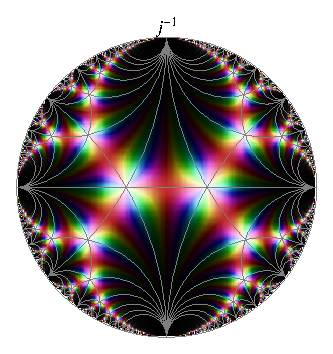
\includegraphics[width=0.45\textwidth]{figures/klein-jinv} & \quad &
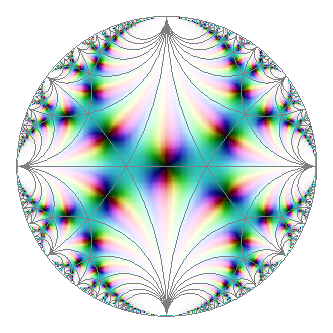
\includegraphics[width=0.45\textwidth]{figures/klein-jm1} \\
\\
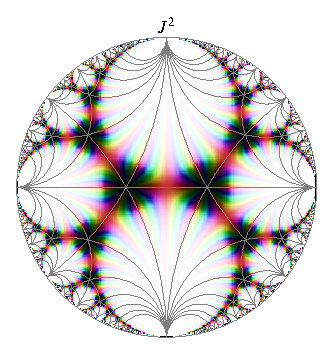
\includegraphics[width=0.45\textwidth]{figures/klein-jsqr} & \quad &
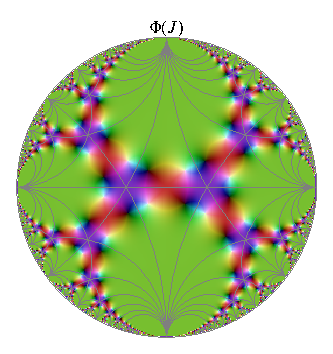
\includegraphics[width=0.45\textwidth]{figures/klein-j-mod-cayley}
\end{tabular}
\caption[Rational functions in $J$]{Examples for rational functions in $J$: The function $z \mapsto \inv{J(z)}$ (top-left) is zero at all rational points (hence the dominant black color) and has a pole of order 3 at all points equivalent to $\rho$. The function $z \mapsto J(z) - 1$ (top-right) has a zero of order 2 at all points equivalent to $\ii$. For $z \mapsto J(z)^2$ (bottom-left), the order of the zeros at points equivalent to $\rho$ is six, \ie twice the order of the zeros of the original function $J$ at that points. Lastly, composing $J$ with the Cayley transform, that is $z \mapsto \ModCayley \circ J(z)$ (bottom-right) yields a zero (\resp pole) of order 1 at every point $z$ for which $J(z) = \ii$ (\resp $J(z) = -\ii$). Its value at rational points is $\ModCayley \circ J(\infty) = \ModCayley(\infty) = \ii$, explaining the dominant green coloring.}
\label{fig_FunctionsOfJ}
\end{figure}
\begin{example}
In Figure~{\ref{fig_FunctionsOfJ}}, four examples for rational functions in $J$ are given. Note that except $z \mapsto J(z)^2$, these maps are instances of modular functions of the form $A \circ J$, where $A$ is a M�bius transformation. 
\end{example}
\clearpage

\begin{figure}
\centering
\includegraphics[width=\textwidth]{figures/klein-jfib-large}
\caption[Klein meets Fibonacci]{The modular function $G = F \circ J$, obtained by composition of the Klein's complete invariant $J$ and the generating function of the Fibonacci sequence, $F(z) = \frac{z}{1 - z - z^2}$, \ie $G(z) = \frac{J(z)}{1 - J(z) - J(z)^2}$, satisfies $G(\infty) = 0$, has zeros of order 3 at all points equivalent to $\rho$ and poles of order 1 at all points $z \in \mathcal{H}$ satisfying $J(z) \in \{-\phi, \reci{\phi}\}$, where $\phi := \frac{1 + \sqrt{5}}{2}$ denotes the golden ratio.}
\label{fig_KleinJFib}
\end{figure}

\begin{example}
\index{Fibonacci sequence}
\index{C-finite sequence}
\index{Generating function}
As a final example, Figure~\ref{fig_KleinJFib} shows what happens, when $J$ is composed with the generating function of the Fibonacci sequence. Although it is a slight digression, we will shortly give some background about the Fibonacci sequence here.

The Fibonacci sequence $0, 1, 1, 2, 3, 5, 8, \dots$ is a so-called \emph{C-finite sequence}, \ie a sequence satisfying a recurrence of the form
\begin{equation*}
\sum_{i=0}^r c_i a_{n+i} = 0 \quad\text{for all $n \ge 0$},
\end{equation*}
where $r$ is the order of the recurrence, $c_i$ are fixed constants and $a_n$ is the $n$-th element of the sequence. The Fibonacci sequence and its elements $F_n$ satisfy the recurrence $F_{n+2} - F_{n+1} - F_n = 0$, $n \ge 0$, with initial values $(F_0,F_1) = (0,1)$. The \emph{generating function} of a sequence $(a_n)_{n\ge 0}$ is defined as
\begin{equation*}
F(z) := \sum_{n \ge 0} a_n z^n.
\end{equation*}
For C-finite sequences, the generating function is always a rational function -- see Theorem 4.3 in \ConcreteTet{}. In particular, the generating function of the Fibonacci sequence is given by
\begin{equation*}
F(z) := \sum_{n \ge 0} F_n z^n = \frac{z}{1 - z - z^2}.
\end{equation*}
More on the topic of sequences and generating functions, as well as symbolic sums and asymptotic estimates may be found in \ConcreteTet{}.
\end{example}
